\documentclass[VM.tex]{subfiles}
\tikzset{
  load/.style   = {ultra thick,-latex},
  stress/.style = {-latex},
  dim/.style    = {latex-latex},
  axis/.style   = {-latex,black!55},
}

% Drawing View
\tikzset{dimetric2/.style={
  x={(0.935cm,-0.28cm)},
  y={(0.44cm, 0.312cm)},
  z={(0.000cm, 0.943cm)},
}}
\begin{document}

\subsubsection*{Description : }
Natural frequency of a square plate is analyzed and compared. 
\subsubsection*{Reference : }
NAFEMS Manual. Solution Retrieved from Ansys verification problem (VMP09-T12).

\subsubsection*{Material and Geometric data : }


\begin{figure}[h!]
\centering
\subfile{VMP09_DRAW.tex}
\caption{VMP09} %\label{VMP09sch}
\end{figure}
\begin{table}[ht]
\renewcommand{\arraystretch}{1.5}
\centering
\caption{Input Data}
%\label{my-labelsdqf}
\begin{tabular}{|ll|ll|ll|}
\hline
\multicolumn{2}{|l|}{\cellcolor[HTML]{C0C0C0}Material Property} & \multicolumn{2}{l|}{\cellcolor[HTML]{C0C0C0}Geometric Data} & \multicolumn{2}{l|}{\cellcolor[HTML]{C0C0C0}Loading Data} \\ \hline  \hline
Young's Modulus ($E$)          & 2E11 $pa$         & Length ($l$)        & 10 $m$        &         &          \\
Poission's Ratio ($\nu$)       & 0.3         & Breath ($b$)        & 10 $m$          &         & Nil       \\ 
Density ($\rho$)       & 8000 $Kg/m^3$         & Thickness($t$)        & 0.05 $m$          &    &        \\ \hline
\end{tabular}
\end{table}




\subsubsection*{Mesh and boundary condition : }



\begin{figure}[h!]
\begin{subfigure}{.45\textwidth}
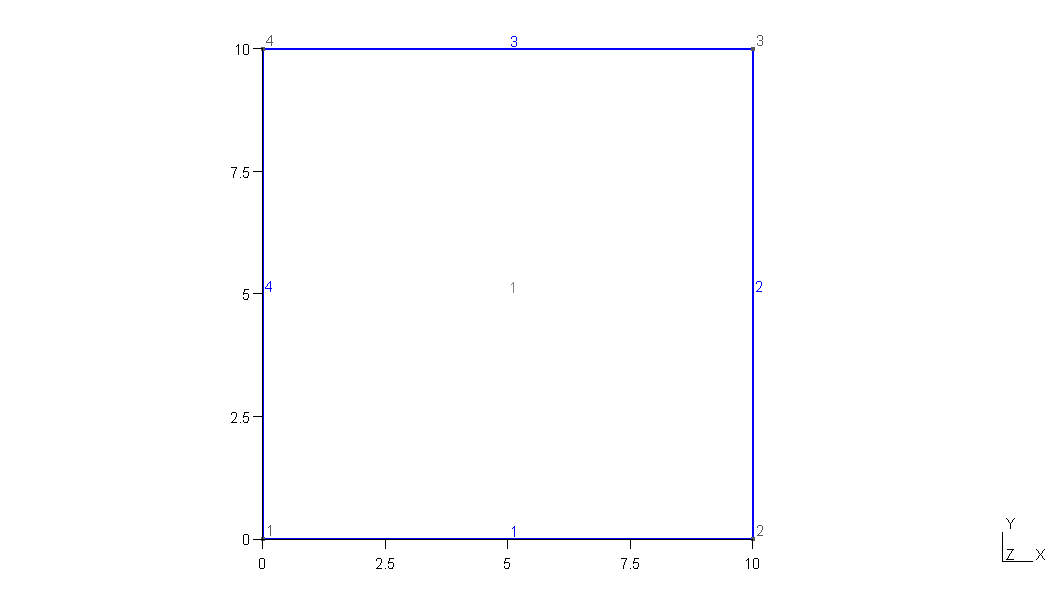
\includegraphics[width=\linewidth,trim={9cm 0 9cm 0},clip]{VMP09/VMP09_T12_geo.png}
%\caption{Mode Shape 4}
\end{subfigure} \hfill
\begin{subfigure}{.45\textwidth}
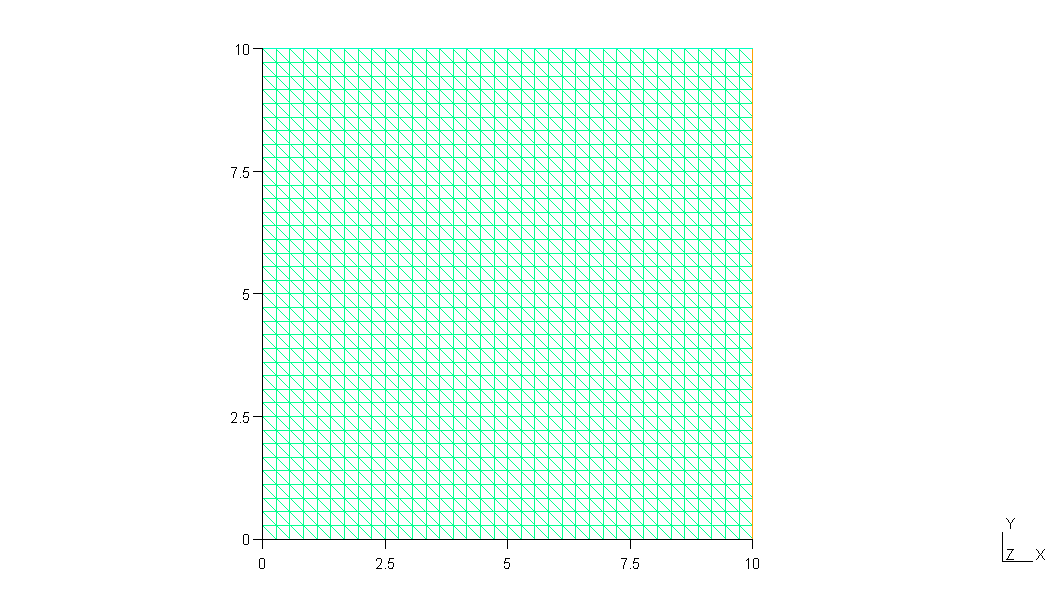
\includegraphics[width=\linewidth,trim={9cm 0 9cm 0},clip]{VMP09/VMP09_T12_msh.png}
%\caption{Mode Shape 5}
\end{subfigure}
\caption{Geomentry and Mesh of TIM68}
\end{figure}








\begin{table}[h!]
\renewcommand{\arraystretch}{1.5}
\centering
\caption{FEM and Boundary condition data}
%\label{my-label}
\begin{tabular}{|l|lll|l|lll|}
\hline
 \multicolumn{4}{l|}{\cellcolor[HTML]{C0C0C0}Direchlet Boundary} & \multicolumn{4}{l|}{\cellcolor[HTML]{C0C0C0}Neumann Boundary} \\ \hline \hline
  Geo - \newline Entity      & $w$          & $\theta _ x$     & $\theta _ y $    & Geo - \newline Entity         & $F_z$        & $M_x$        & $M_y$        \\ \hline
 line \{1,2,3,4\}     & Free  & Free   & Free &Nil                    &         &           &           \\ \hline
\end{tabular}
\end{table}
\subsubsection*{Analytically solution : }
Retrieved Natural frequencies from reference manuals are \\
Mode 4 = 1.622 $Hz$ \\
Mode 5 = 2.360 $Hz$ \\
Mode 6 = 2.922 $Hz$ \\
Mode 7 = 4.233 $Hz$ \\
Mode 8 = 4.233 $Hz$ \\
Mode 9 = 7.416 $Hz$ \\

\subsubsection*{Result and error analysis : }
The Natural modes obtained are plotted in the below figures. 


\begin{figure}[h!]
\begin{subfigure}{.3\textwidth}
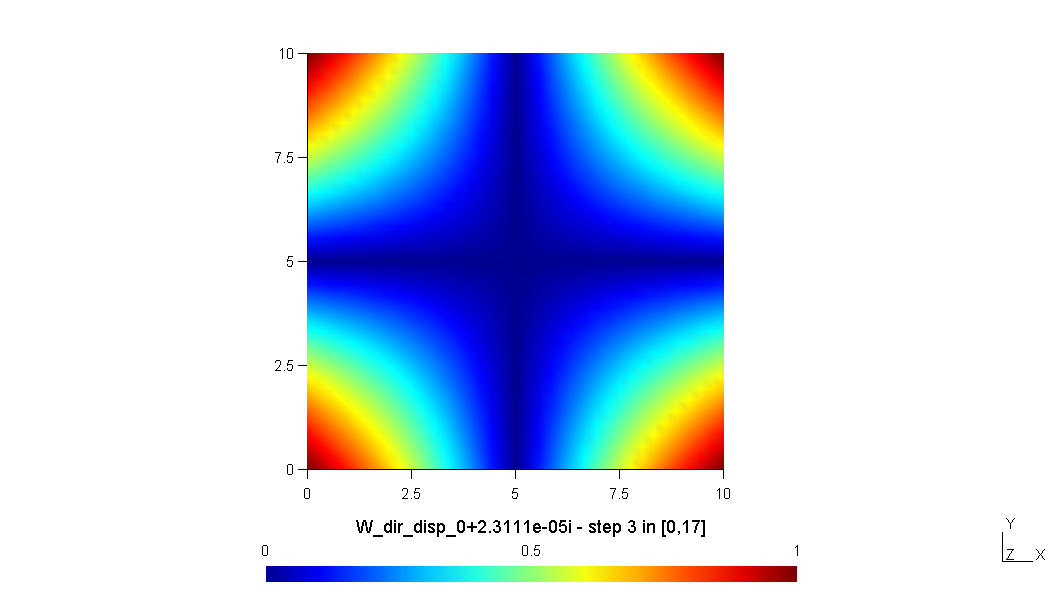
\includegraphics[width=\linewidth,trim={8cm 0 8cm 0},clip]{VMP09/VMP09_T12_pos_F4.png}
\caption{Mode Shape 4}
\end{subfigure} \hfill
\begin{subfigure}{.3\textwidth}
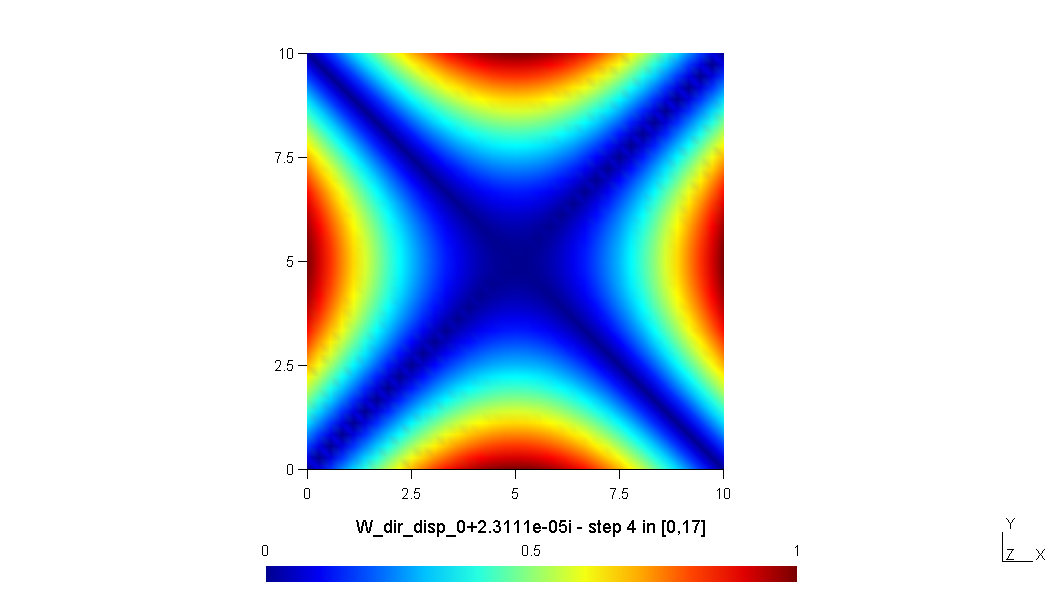
\includegraphics[width=\linewidth,trim={8cm 0 8cm 0},clip]{VMP09/VMP09_T12_pos_F5.png}
\caption{Mode Shape 5}
\end{subfigure}\hfill
\begin{subfigure}{.3\textwidth}
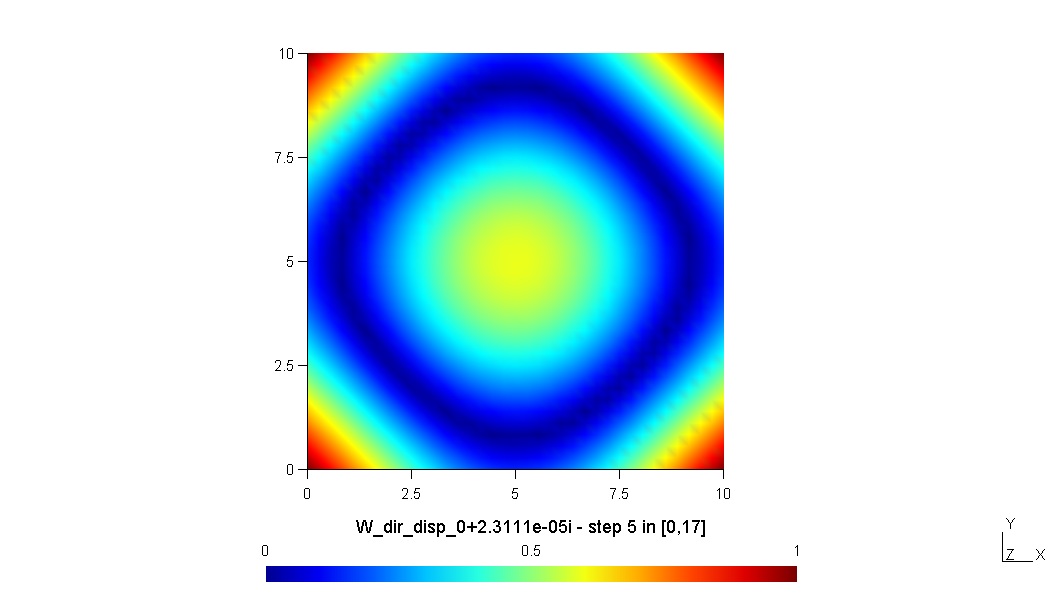
\includegraphics[width=\linewidth,trim={8cm 0 8cm 0},clip]{VMP09/VMP09_T12_pos_F6.png}
\caption{Mode Shape 6}
\end{subfigure}\vfill
\begin{subfigure}{.3\textwidth}
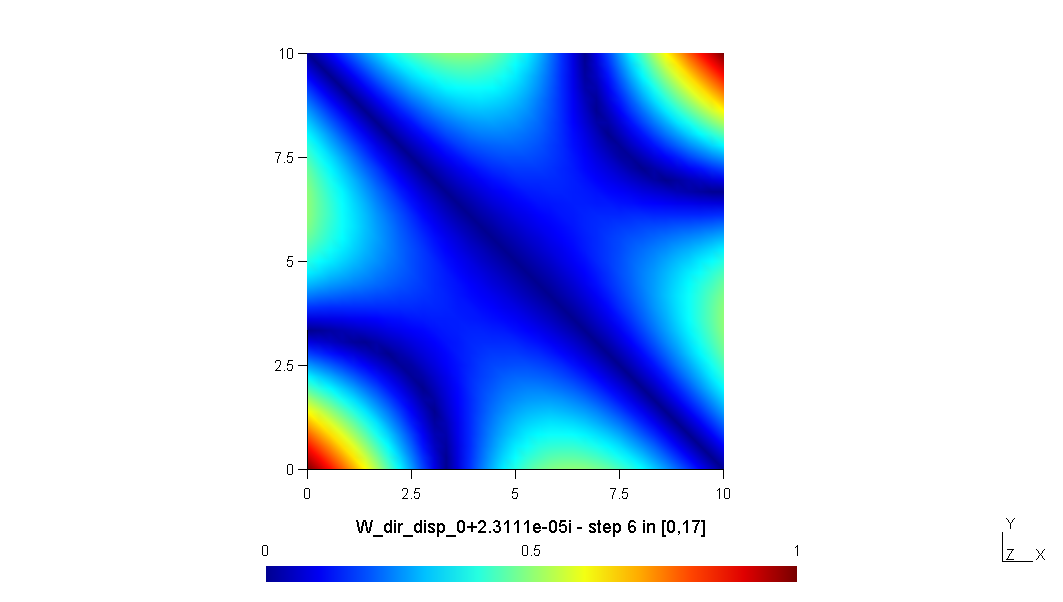
\includegraphics[width=\linewidth,trim={8cm 0 8cm 0},clip]{VMP09/VMP09_T12_pos_F7.png}
\caption{Mode Shape 7}
\end{subfigure} \hfill
\begin{subfigure}{.3\textwidth}
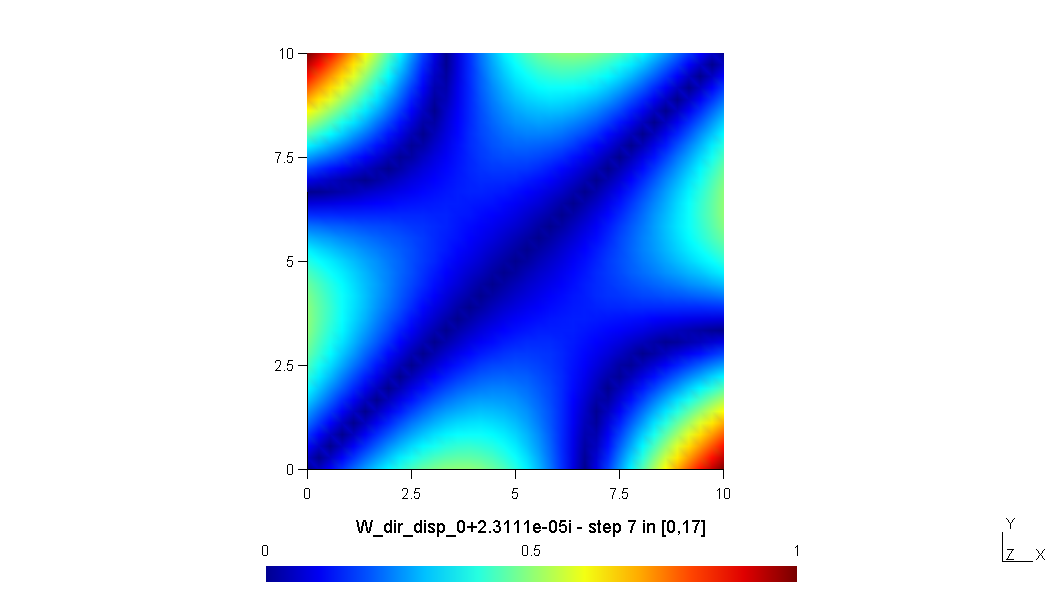
\includegraphics[width=\linewidth,trim={8cm 0 8cm 0},clip]{VMP09/VMP09_T12_pos_F8.png}
\caption{Mode Shape 8}
\end{subfigure}\hfill
\begin{subfigure}{.3\textwidth}
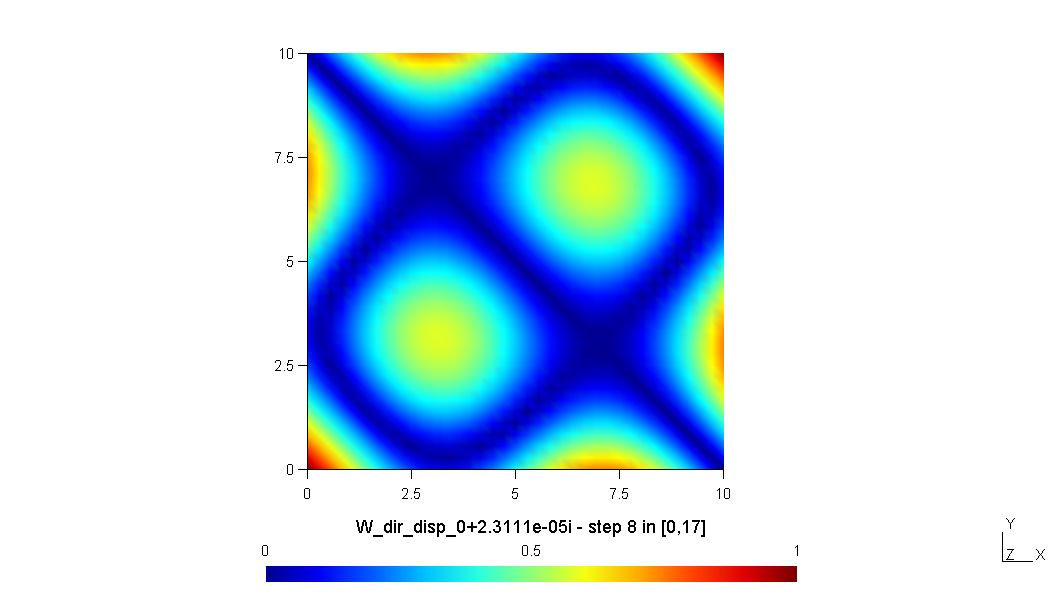
\includegraphics[width=\linewidth,trim={8cm 0 8cm 0},clip]{VMP09/VMP09_T12_pos_F9.png}
\caption{Mode Shape 9}
\end{subfigure}
\caption{Natural Modes of a Square Plate}
\end{figure}

For each natural frequency the error percentage is \\
Mode 4 =  0.0018 $\%$ \\
Mode 5 =  0.0042 $\%$ \\
Mode 6 =  0.061 $\%$ \\ 
Mode 7 =  0.911 $\%$ \\
Mode 8 =  0.902 $\%$ \\
Mode 9 =  0.645 $\%$ \\




%%%%% scrap
\begin{comment}

\end{comment}








\end{document}